%%%%%%%%%%%%%%%%%%%%%%%%%%%%%%%%%%%%%%%%%
% Short Sectioned Assignment
% LaTeX Template
% Version 1.0 (5/5/12)
%
% This template has been downloaded from:
% http://www.LaTeXTemplates.com
%
% Original author:
% Frits Wenneker (http://www.howtotex.com)
%
% License:
% CC BY-NC-SA 3.0 (http://creativecommons.org/licenses/by-nc-sa/3.0/)
%
%%%%%%%%%%%%%%%%%%%%%%%%%%%%%%%%%%%%%%%%%

%----------------------------------------------------------------------------------------
%	PACKAGES AND OTHER DOCUMENT CONFIGURATIONS
%----------------------------------------------------------------------------------------

\documentclass[paper=a4, fontsize=11pt]{scrartcl} % A4 paper and 11pt font size

\usepackage[T1]{fontenc} % Use 8-bit encoding that has 256 glyphs
\usepackage{fourier} % Use the Adobe Utopia font for the document - comment this line to return to the LaTeX default
\usepackage[english]{babel} % English language/hyphenation
\usepackage{amsmath,amsfonts,amsthm} % Math packages
\usepackage{listings} % Required for insertion of code
\usepackage{sectsty} % Allows customizing section commands
\allsectionsfont{\centering \normalfont\scshape} % Make all sections centered, the default font and small caps
\usepackage{graphicx}
\usepackage{fancyhdr} % Custom headers and footers
\pagestyle{fancyplain} % Makes all pages in the document conform to the custom headers and footers
\fancyhead{} % No page header - if you want one, create it in the same way as the footers below
\fancyfoot[L]{} % Empty left footer
\fancyfoot[C]{} % Empty center footer
\fancyfoot[R]{\thepage} % Page numbering for right footer
\renewcommand{\headrulewidth}{0pt} % Remove header underlines
\renewcommand{\footrulewidth}{0pt} % Remove footer underlines
\setlength{\headheight}{13.6pt} % Customize the height of the header

\numberwithin{equation}{section} % Number equations within sections (i.e. 1.1, 1.2, 2.1, 2.2 instead of 1, 2, 3, 4)
\numberwithin{figure}{section} % Number figures within sections (i.e. 1.1, 1.2, 2.1, 2.2 instead of 1, 2, 3, 4)
\numberwithin{table}{section} % Number tables within sections (i.e. 1.1, 1.2, 2.1, 2.2 instead of 1, 2, 3, 4)

\setlength\parindent{0pt} % Removes all indentation from paragraphs - comment this line for an assignment with lots of text

%----------------------------------------------------------------------------------------
%	CODE INCLUSION CONFIGURATION
%---------------------------------------------------------------------------------------
\lstset{caption=Algorithm 1,
        language = java,
        frame=single, % Single frame around code      
}

%----------------------------------------------------------------------------------------
%	TITLE SECTION
%----------------------------------------------------------------------------------------

\newcommand{\horrule}[1]{\rule{\linewidth}{#1}} % Create horizontal rule command with 1 argument of height

\title{	
\normalfont \normalsize
\textsc{Indiana University, School of Informatics and Computing} \\ [25pt] % Your university, school and/or department name(s)
\horrule{0.5pt} \\[0.4cm] % Thin top horizontal rule
\huge Distributed Systems \\ % The assignment title
\huge Project 1 \\ % The assignment title
\normalsize(Due Sept 11th, 2016)
\horrule{2pt} \\[0.5cm] % Thick bottom horizontal rule
}

\author{Ethan Li, Rohit Patil} % Your name

\date{} % Today's date or a custom date

\begin{document}
\maketitle % Print the title

%----------------------------------------------------------------------------------------
 

\textbf{The description of the main steps and data flow in your program.}\\

There are three main steps.\\

The first main step is to load the data from the input file. The data is stored in a HashMap with the formation of adjacency matrix.  The keys in the hashmap are URLs and the values are the outgoing URLs associated with the keys. \\

The second step is calculation. It will calculate page rank values for M times set by users. In a single iteration, for URLs with outgoing urls, their values will be set by the values of their outgoing urls. For example, if url 1 has two outgoing urls which are url 2 and url 3, then \\
prNew(1) = (1-d) / N + d * ( pr(2)/L(2) + pr(3)/L(3) + danglingValue). \\
Here, prNew(i) is the new rank value of URL i, pr(i) is the previous rank value of URL i, L(i) is the out-degree of URL i, N is the number of URLs, d is damping factor, and danglingValue is the sum of the previous rank values of all dangling nodes divided by N. For those dangling nodes, their new page rank values are  prNew = (1-d) / N + d * (danglingValue). After M iterations, the page rank values are recalculated and towards to convergence.\\

Finally, sorting the URLs by their ranks. And then output the top 10 with their rank values to a file.\\

In this process, the data is read from input file and being stored and calculated in memory, then written back to disk.\\



\textbf{The output is:}
\begin{figure}[htbp]
\centering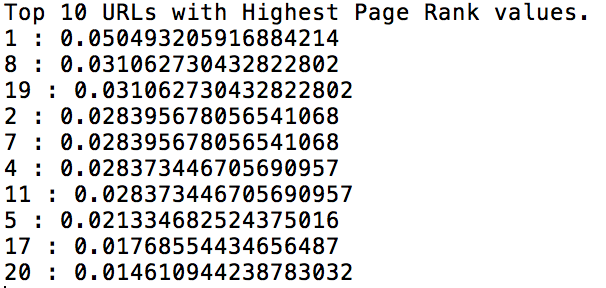
\includegraphics[width=3.5in]{output.png}
\caption{The top 10 URLs in pagerank.input.1000.urls.19 file }\label{Gorilla}
\end{figure}
 
 





%----------------------------------------------------------------------------------------

\end{document}